\documentclass{article}

% if you need to pass options to natbib, use, e.g.:
%     \PassOptionsToPackage{numbers, compress}{natbib}
% before loading neurips_2020

% ready for submission
% \usepackage{neurips_2020}

% to compile a preprint version, e.g., for submission to arXiv, add add the
% [preprint] option:
%     \usepackage[preprint]{neurips_2020}

% to compile a camera-ready version, add the [final] option, e.g.:
%     \usepackage[final]{neurips_2020}

% to avoid loading the natbib package, add option nonatbib:
\usepackage{format}

\usepackage[utf8]{inputenc} % allow utf-8 input
\usepackage[T1]{fontenc}    % use 8-bit T1 fonts
\usepackage{hyperref}       % hyperlinks
\usepackage{url}            % simple URL typesetting
\usepackage{booktabs}       % professional-quality tables
\usepackage{amsfonts}       % blackboard math symbols
\usepackage{nicefrac}       % compact symbols for 1/2, etc.
\usepackage{microtype}      % microtypography
\usepackage{graphicx}
\usepackage{xcolor}
\hypersetup{
	colorlinks,
	linkcolor={red!50!black},
	citecolor={blue!50!black},
	urlcolor={blue!80!black}
}

\title{Abstract vector sketch generation using differentiable rendering and GANs}

% The \author macro works with any number of authors. There are two commands
% used to separate the names and addresses of multiple authors: \And and \AND.
%
% Using \And between authors leaves it to LaTeX to determine where to break the
% lines. Using \AND forces a line break at that point. So, if LaTeX puts 3 of 4
% authors names on the first line, and the last on the second line, try using
% \AND instead of \And before the third author name.

\author{
   Ivan Puhachov \\ 
   UdeM \\
   ivan.puhachov@umontreal.ca \\
}

\begin{document}

\maketitle

\begin{abstract}
  The abstract paragraph is \emph{optional} for the extended abstract and \emph{mandatory} in the final project report.
\end{abstract}

\section{Overview}
Drawings are an important part of creative processes - we draw to discuss ideas, express emotions, outline a prototype. However, drawings are hard to process by machine as they use high-level abstractions to convey shapes and depth information, support structures and auxiliary lines (see Figure \ref{fig:designsketch} for reference). But that's what make sketches interesting, as they are inexact depiction of familiar objects.

Sketch generation is a known problem, however less popular than general image generation, because less training data is available. Another problem for generation is data representation: digital drawings are often stored in the SVG (scalable vector graphics) format, when we store individual strokes and shapes as mathematical expressions. This allows for scaling and editing without loss in quality, opposed to raster format (storing pixels). To visualize vector graphics (and compare it with target image, for example) we need a rasterizer, and for deep learning applications we need a differentiable rasterizer. 





\subsection{Idea}

\paragraph{Hypothesis}

\section{Implementation details}

\paragraph{Third-party code} I will use differentiable rendering from \cite{diffsvg} available at: \href{https://github.com/BachiLi/diffvg}{github}. I will also use third-party datasets from Sketch-RNN \cite{sketchrnn} and DoodlerGAN \cite{doodlergan} for experimenting.

\paragraph{Github} I will \href{https://github.com/ivanpuhachov/ift6756}{personal github repo}

\paragraph{Resources} I will use my machine with NVidia 2080Ti GPU (11 GB) and Google Colab to run experiments in parallel.

\section{Guidelines Extended Abstract and Final Project Report}

\subsection{Timeline -- Dates Importantes}
\begin{itemize}
    \item March 13th (11:59PM \href{https://www.timeanddate.com/time/zones/aoe}{AoE}): Extended Abstract submission -- Soumission du pré-rapport (\textbf{max 2 pages}).
    \item April 23rd (11:59PM \href{https://www.timeanddate.com/time/zones/aoe}{AoE}): Project Report submission -- Soumission du rapport de projet (\textbf{max 8 pages}).
    \item End of April: Project Presentations (Optional if a paper presentation has already been done) -- Présentation des projets (facultative si une présentation de papier à déjà été faite)
\end{itemize}

\paragraph{Penalty policy:} 10\% of the grade per 24h late. Example: you submit March 14th at 1:00AM (AoE) you get a penalty of 10\%. You submit March 15th at 2:00AM (AoE) you get a penalty of 20\%.

Note that each time you edit your submission it \emph{removes} the previous timestamp. 

\subsection{Details}
The goal of the extended abstract is to separate the generation and confirmation of hypotheses. This process is inspired from the \href{https://preregister.science/}{Pre-registation experiement NeurIPS 2020 workshop.} The idea is to separate the formulation of a scientific hypothesis to its validation: 
\begin{center}
\begin{minipage}{ .9\textwidth}
\emph{Pre-registration changes the incentives by reviewing [...] before experiments are conducted. The emphasis will be on whether the experiment plan can adequately prove or disprove one (or more) hypotheses. Some results will be negative, and this is welcomed. This way, good ideas that do not work will get welcomed. Finally, the clear separation between hypothesizing and confirmation will raise the statistical significance of the results.}
\end{minipage}
\end{center}
As a summary the process is:
\begin{itemize}
    \item Come up with a project (empirical or theoretical). The goal here is to pinpoint new questions.
    \item Write the extended abstract without confirmatory experiments/proofs by motivating this idea. (Providing context and motivations) 
    \item Run the experiments/work on the proofs and report your results.
\end{itemize}

    
\subsection{Pages limits}

The extended abstract should be \textbf{maximum 2 pages long} (not including refs) and the final report should be \textbf{maximum 8 pages long} (not including refs). You can also have an appendix for proofs and additional results but the focus of the evaluation will be on the 8 pages of the main text.

\subsection{Code}

The code can be an important aspect of the project. If it is the case it \emph{must} be part of the project report. The source can be shared with the project report but it is strongly advised to share a Github repository (or any other version control system) containing the frequent commits of code. Here is a summary of the guidelines:
\begin{enumerate}
    \item A good practice is to start a Github repository as soon as possible and to frequently commit you updates on the code.
    \item I advice you to use a strong IDE (integrated development environment). My advice is \href{https://www.jetbrains.com/community/education/#students}{Pycharm} (you can get a free license as a student). 
    \item It is fine to use some open source code if you are transparent about it! (If you pretend it is your own code it is considered as plagiarism) 
    \item 
	If you need advice about the coding workflow/good practices come to the office hours.
\end{enumerate}

Regarding the project contributions, doing a new experiment that is well motivated and requires the design of some new code is a sufficient contribution for the project. The motivations and descriptions of the new experiment(s) should be presented in the extended abstract.

\subsection{Resources}

In order to access the feasibility of your project. You should roughly indicate the computational resources you will have access to (cluster, personal GPU, collab,...)
% \section{General formatting instructions}
% \label{gen_inst}

% The text must be confined within a rectangle 5.5~inches (33~picas) wide and
% 9~inches (54~picas) long. The left margin is 1.5~inch (9~picas).  Use 10~point
% type with a vertical spacing (leading) of 11~points.  Times New Roman is the
% preferred typeface throughout, and will be selected for you by default.
% Paragraphs are separated by \nicefrac{1}{2}~line space (5.5 points), with no
% indentation.

% The paper title should be 17~point, initial caps/lower case, bold, centered
% between two horizontal rules. The top rule should be 4~points thick and the
% bottom rule should be 1~point thick. Allow \nicefrac{1}{4}~inch space above and
% below the title to rules. All pages should start at 1~inch (6~picas) from the
% top of the page.

% For the final version, authors' names are set in boldface, and each name is
% centered above the corresponding address. The lead author's name is to be listed
% first (left-most), and the co-authors' names (if different address) are set to
% follow. If there is only one co-author, list both author and co-author side by
% side.

% Please pay special attention to the instructions in Section \ref{others}
% regarding figures, tables, acknowledgments, and references.

% \section{Headings: first level}
% \label{headings}

% All headings should be lower case (except for first word and proper nouns),
% flush left, and bold.

% First-level headings should be in 12-point type.

% \subsection{Headings: second level}

% Second-level headings should be in 10-point type.

% \subsubsection{Headings: third level}

% Third-level headings should be in 10-point type.

% \paragraph{Paragraphs}

% There is also a \verb+\paragraph+ command available, which sets the heading in
% bold, flush left, and inline with the text, with the heading followed by 1\,em
% of space.

% \section{Citations, figures, tables, references}
% \label{others}

% These instructions apply to everyone.

% \subsection{Citations within the text}

% The \verb+natbib+ package will be loaded for you by default.  Citations may be
% author/year or numeric, as long as you maintain internal consistency.  As to the
% format of the references themselves, any style is acceptable as long as it is
% used consistently.

% The documentation for \verb+natbib+ may be found at
% \begin{center}
%   \url{http://mirrors.ctan.org/macros/latex/contrib/natbib/natnotes.pdf}
% \end{center}
% Of note is the command \verb+\citet+, which produces citations appropriate for
% use in inline text.  For example,
% \begin{verbatim}
%   \citet{hasselmo} investigated\dots
% \end{verbatim}
% produces
% \begin{quote}
%   Hasselmo, et al.\ (1995) investigated\dots
% \end{quote}

% If you wish to load the \verb+natbib+ package with options, you may add the
% following before loading the \verb+neurips_2020+ package:
% \begin{verbatim}
%   \PassOptionsToPackage{options}{natbib}
% \end{verbatim}

% If \verb+natbib+ clashes with another package you load, you can add the optional
% argument \verb+nonatbib+ when loading the style file:
% \begin{verbatim}
%   \usepackage[nonatbib]{format}
% \end{verbatim}

% As submission is double blind, refer to your own published work in the third
% person. That is, use ``In the previous work of Jones et al.\ [4],'' not ``In our
% previous work [4].'' If you cite your other papers that are not widely available
% (e.g., a journal paper under review), use anonymous author names in the
% citation, e.g., an author of the form ``A.\ Anonymous.''

% \subsection{Footnotes}

% Footnotes should be used sparingly.  If you do require a footnote, indicate
% footnotes with a number\footnote{Sample of the first footnote.} in the
% text. Place the footnotes at the bottom of the page on which they appear.
% Precede the footnote with a horizontal rule of 2~inches (12~picas).

% Note that footnotes are properly typeset \emph{after} punctuation
% marks.\footnote{As in this example.}

% \subsection{Figures}

% \begin{figure}
%   \centering
%   \fbox{\rule[-.5cm]{0cm}{4cm} \rule[-.5cm]{4cm}{0cm}}
%   \caption{Sample figure caption.}
% \end{figure}

% All artwork must be neat, clean, and legible. Lines should be dark enough for
% purposes of reproduction. The figure number and caption always appear after the
% figure. Place one line space before the figure caption and one line space after
% the figure. The figure caption should be lower case (except for first word and
% proper nouns); figures are numbered consecutively.

% You may use color figures.  However, it is best for the figure captions and the
% paper body to be legible if the paper is printed in either black/white or in
% color.

% \subsection{Tables}

% All tables must be centered, neat, clean and legible.  The table number and
% title always appear before the table.  See Table~\ref{sample-table}.

% Place one line space before the table title, one line space after the
% table title, and one line space after the table. The table title must
% be lower case (except for first word and proper nouns); tables are
% numbered consecutively.

% Note that publication-quality tables \emph{do not contain vertical rules.} We
% strongly suggest the use of the \verb+booktabs+ package, which allows for
% typesetting high-quality, professional tables:
% \begin{center}
%   \url{https://www.ctan.org/pkg/booktabs}
% \end{center}
% This package was used to typeset Table~\ref{sample-table}.

% \begin{table}
%   \caption{Sample table title}
%   \label{sample-table}
%   \centering
%   \begin{tabular}{lll}
%     \toprule
%     \multicolumn{2}{c}{Part}                   \\
%     \cmidrule(r){1-2}
%     Name     & Description     & Size ($\mu$m) \\
%     \midrule
%     Dendrite & Input terminal  & $\sim$100     \\
%     Axon     & Output terminal & $\sim$10      \\
%     Soma     & Cell body       & up to $10^6$  \\
%     \bottomrule
%   \end{tabular}
% \end{table}

% \section{Final instructions}

% Do not change any aspects of the formatting parameters in the style files.  In
% particular, do not modify the width or length of the rectangle the text should
% fit into, and do not change font sizes (except perhaps in the
% \textbf{References} section; see below). Please note that pages should be
% numbered.

% \section{Preparing PDF files}

% Please prepare submission files with paper size ``US Letter,'' and not, for
% example, ``A4.''

% Fonts were the main cause of problems in the past years. Your PDF file must only
% contain Type 1 or Embedded TrueType fonts. Here are a few instructions to
% achieve this.

% \begin{itemize}

% \item You should directly generate PDF files using \verb+pdflatex+.

% \item You can check which fonts a PDF files uses.  In Acrobat Reader, select the
%   menu Files$>$Document Properties$>$Fonts and select Show All Fonts. You can
%   also use the program \verb+pdffonts+ which comes with \verb+xpdf+ and is
%   available out-of-the-box on most Linux machines.

% \item The IEEE has recommendations for generating PDF files whose fonts are also
%   acceptable for NeurIPS. Please see
%   \url{http://www.emfield.org/icuwb2010/downloads/IEEE-PDF-SpecV32.pdf}

% \item \verb+xfig+ "patterned" shapes are implemented with bitmap fonts.  Use
%   "solid" shapes instead.

% \item The \verb+\bbold+ package almost always uses bitmap fonts.  You should use
%   the equivalent AMS Fonts:
% \begin{verbatim}
%   \usepackage{amsfonts}
% \end{verbatim}
% followed by, e.g., \verb+\mathbb{R}+, \verb+\mathbb{N}+, or \verb+\mathbb{C}+
% for $\mathbb{R}$, $\mathbb{N}$ or $\mathbb{C}$.  You can also use the following
% workaround for reals, natural and complex:
% \begin{verbatim}
%   \newcommand{\RR}{I\!\!R} %real numbers
%   \newcommand{\Nat}{I\!\!N} %natural numbers
%   \newcommand{\CC}{I\!\!\!\!C} %complex numbers
% \end{verbatim}
% Note that \verb+amsfonts+ is automatically loaded by the \verb+amssymb+ package.

% \end{itemize}

% If your file contains type 3 fonts or non embedded TrueType fonts, we will ask
% you to fix it.

% \subsection{Margins in \LaTeX{}}

% Most of the margin problems come from figures positioned by hand using
% \verb+\special+ or other commands. We suggest using the command
% \verb+\includegraphics+ from the \verb+graphicx+ package. Always specify the
% figure width as a multiple of the line width as in the example below:
% \begin{verbatim}
%   \usepackage[pdftex]{graphicx} ...
%   \includegraphics[width=0.8\linewidth]{myfile.pdf}
% \end{verbatim}
% See Section 4.4 in the graphics bundle documentation
% (\url{http://mirrors.ctan.org/macros/latex/required/graphics/grfguide.pdf})

% A number of width problems arise when \LaTeX{} cannot properly hyphenate a
% line. Please give LaTeX hyphenation hints using the \verb+\-+ command when
% necessary.


% \section*{Broader Impact}

% Authors are encouraged to include a statement of the broader impact of their work, including its ethical aspects and future societal consequences. 
% Authors should discuss both positive and negative outcomes, if any. For instance, authors should discuss a) 
% who may benefit from this research, b) who may be put at disadvantage from this research, c) what are the consequences of failure of the system, and d) whether the task/method leverages
% biases in the data. If authors believe this is not applicable to them, authors can simply state this.

% Use unnumbered first level headings for this section, which should go at the end of the report. {\bf Note that this section does not count towards the eight pages of content that are allowed.}

\pagebreak
\section*{References}

\bibliography{example_paper}
\bibliographystyle{abbrvnat}


\appendix 
\section{Figures}
\begin{figure}[h]
	\centering
	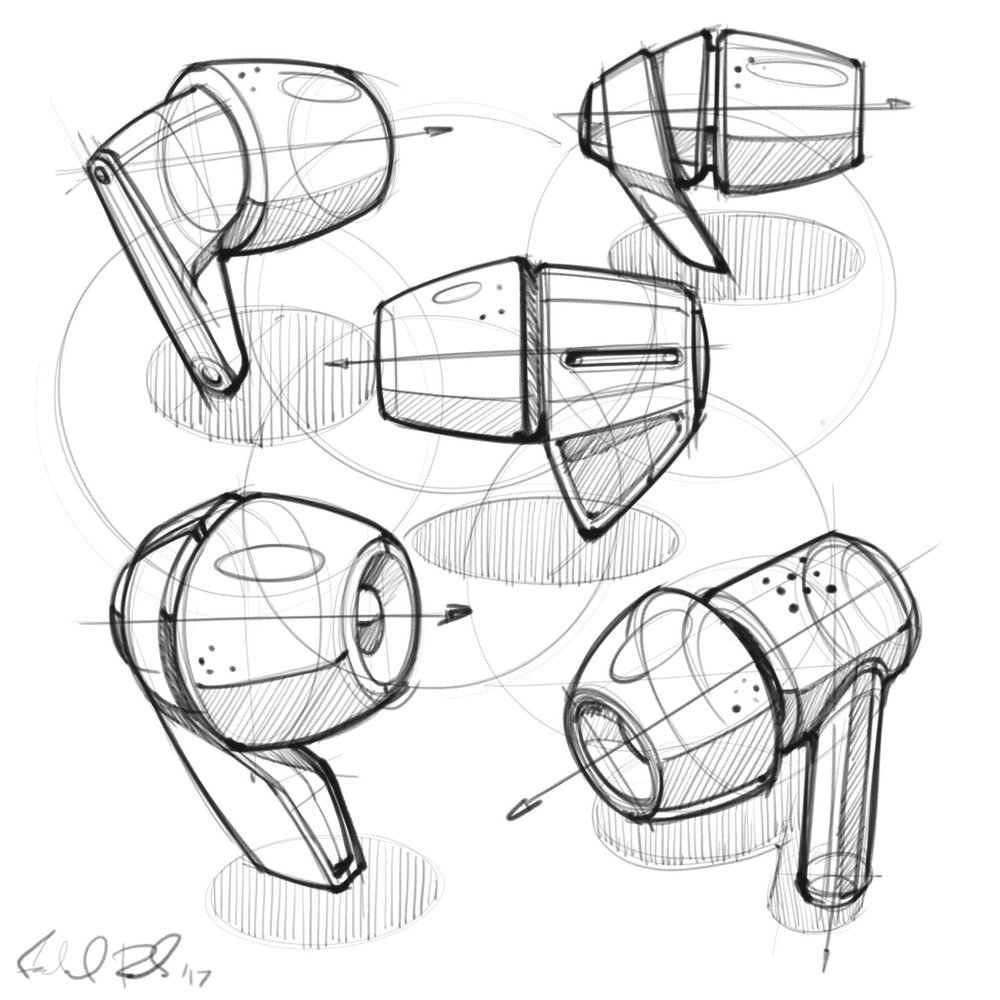
\includegraphics[width=0.55\textwidth]{img/sketch.jpeg}
	\caption{Example of a design sketch. Source: \href{https://fedriosdesign.com/design-sketching}{fedriodesign}}
	\label{fig:designsketch}
\end{figure}
\begin{figure}[h]
	\centering
	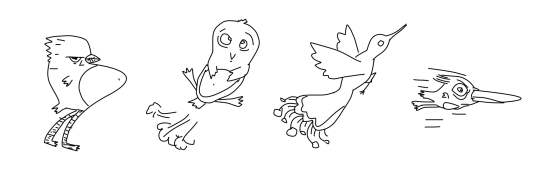
\includegraphics[width=0.55\textwidth]{img/doodlergan1.png}
	\caption{Example of a design sketch}
	\label{fig:doodlergan}
\end{figure}
\end{document}